\chapter{Detector Calibration System}

To run an experiment like CUORE, precise understanding of the energies of each event is necessary, particularly in order to reach the design goal of 5 keV energy resolution.
Due to the complicated behavior of the crystals \color{red} add more here, possibly about the thermal model \color{black}, the thermal response to energy depositions needs to be characterized over multiple energies for each of the 988 TeO$_2$ crystals in CUORE.
This is done by occasionally inserting radioactive sources with known intensity and composition, viz. $^{232}$Th, that emit mono-energetic particles such as photons that will deposit energy into the detectors.
The thermal response of the detectors can then be mapped one-to-one with these known energies, and thus the entire detector array can be individually calibrated.

\section{Overview}

Making such a system, however, is an enormous technical challenge.
In CUORE-0 and Cuoricino, calibration sources could be deployed by hand inside the innermost lead shielding to irradiate a single tower of detectors, see \autoref{fig:CUORE-0_cryostat_schematic}.
However, with 19 towers of crystals making up the CUORE detector array, and with thicker layers of shielding, efficiently deploying sources inside the cryostat requires the sources to be placed in between the towers and inside the roman lead shielding.
This significantly adds to the challenge of such a system as the calibration sources need to be both inserted and retracted from the coldest region of the cryostat on a regular basis.
The main challenges can be summarized as follows: 
\begin{itemize}
\item Calibrate all 988 crystals in as short a time as possible
\item Minimize thermal disturbance to the crystat and the crystals
\item Negligibly contribute to the background in operation
\end{itemize}

The solution to these issues was the Detector Calibration System developed at Wisconsin and at Yale.
With this system, shown in \autoref{fig:DCSintegration}, 12 kevlar strings containing copper capsules with 2\% thoriated tungsten wire are inserted into the cryostat from 300~K down into the detector region at 10 and 50 mK. 

\begin{figure}[htbp]
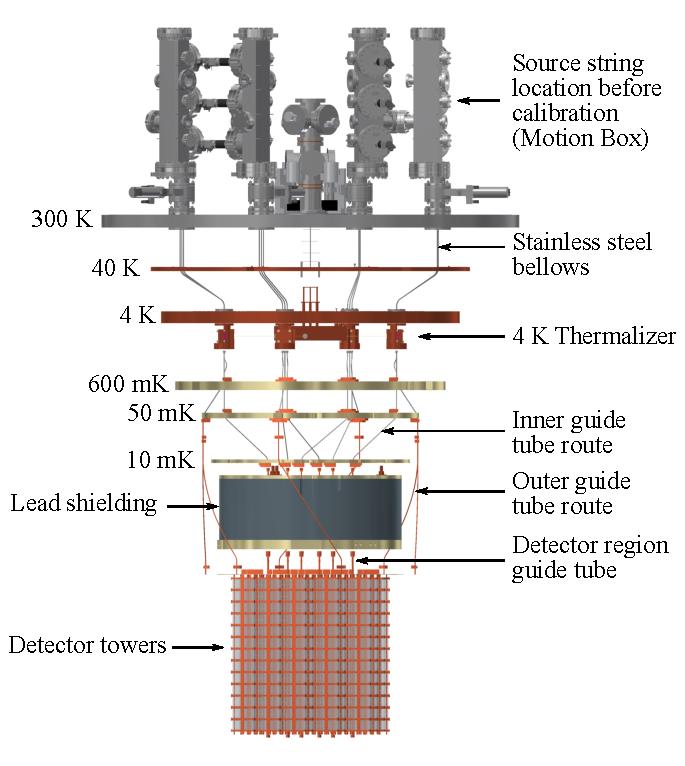
\includegraphics[width=\linewidth]{Figures/DCSintegration.pdf}
\caption[The CUORE Detector Calibration System (DCS).]
{The CUORE Detector Calibration System (DCS).
12 kevlar strings are deployed intermittently into the cryostat through individual tubes through the stages of the cryostat. 6 of the strings are deployed through the inner guide tubes into the 10 mK region of the cryostat between the detector towers, and the other 6 strings are deployed outside the towers in the 50 mK region.}
\label{fig:DCSintegration}
\end{figure}

\section{Calibration Hardware}

figures to add here: Diagram of full calibration system, diagram of all the calibration tubes and paths

\begin{figure}[htbp]
    \centering
    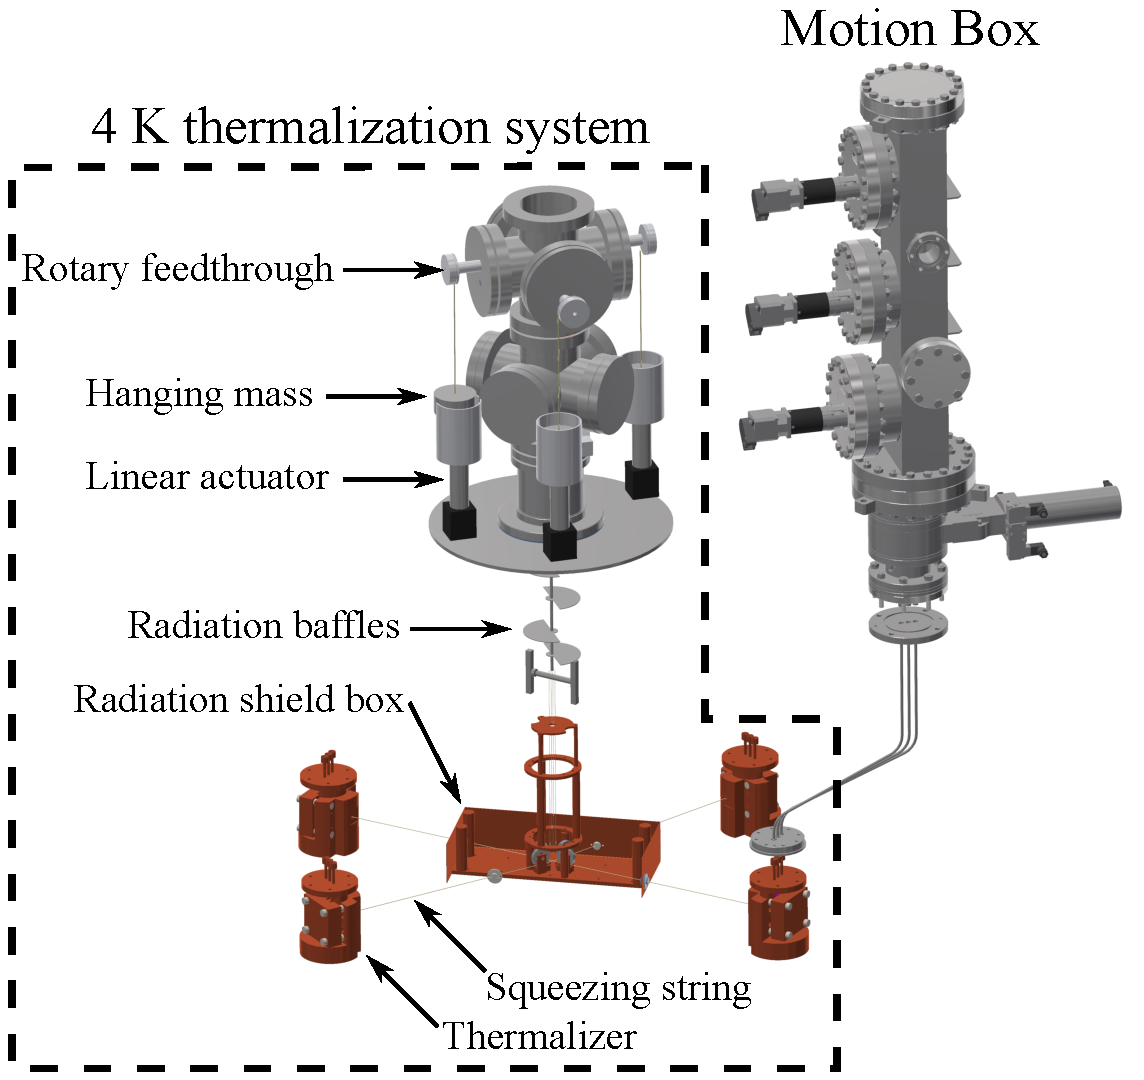
\includegraphics[width=0.8\linewidth]{Figures/thermalization_system_labeled.pdf}
    \caption{Caption}
    \label{fig:DCS_4K_thermalizer}
\end{figure}

\begin{figure}[htbp]
    \centering
    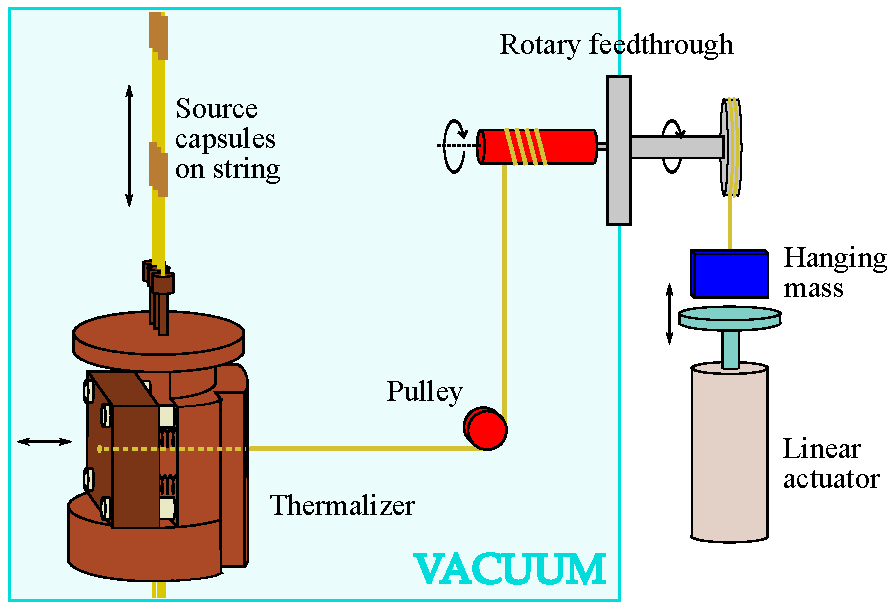
\includegraphics[width=0.8\linewidth]{Figures/Thermalizer_schematic_labeled.pdf}
    \caption{Caption}
    \label{fig:DCS_4K_schematic}
\end{figure}

\begin{figure}[htbp]
    \centering
    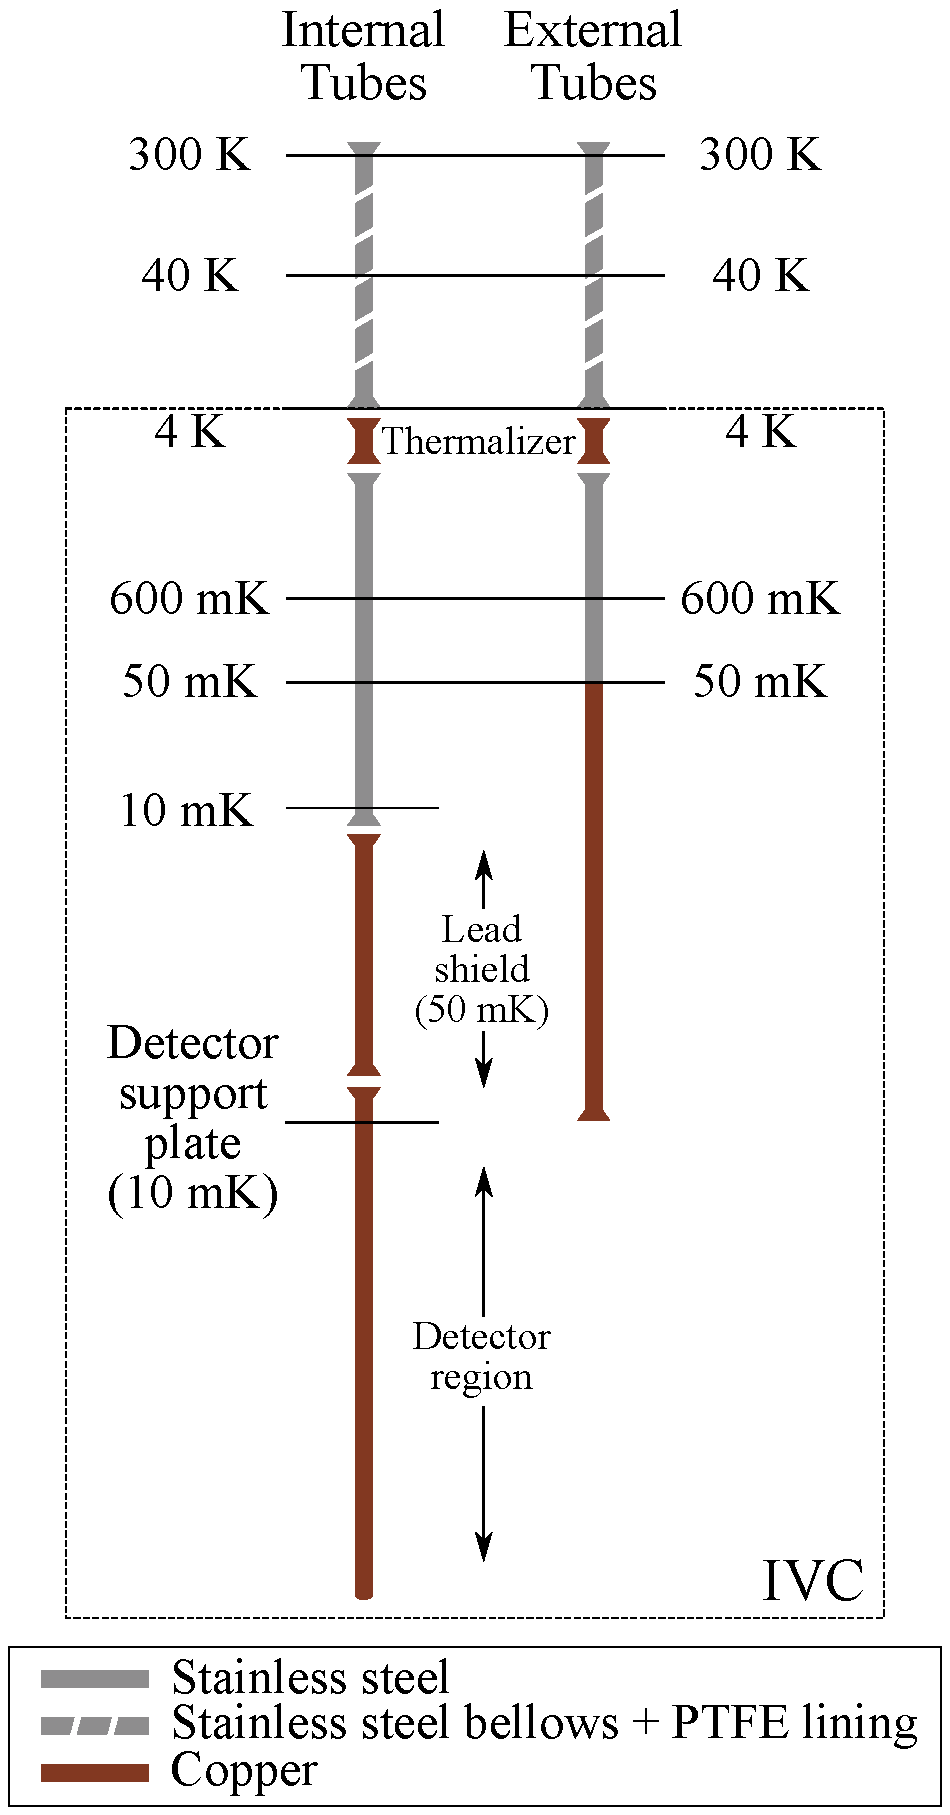
\includegraphics[height=0.4\paperheight]{Figures/thermal_coupling.pdf}
    \caption[A diagram showing the thermal couplings of the DCS tubes for both the internal and external sources.]
    {A diagram showing the thermal couplings of the DCS tubes for both the internal and external sources.
    In order to minimize the thermal load on the cryostat, there are multiple breaks in the DCS tubes with funnels for the calibration sources to pass through.
    Near the detectors, the tubes switch from being stainless steel with low thermal conductivity to low-background copper.
    For the external tubes, there are no tubes below the lead shield and the source capsules hang freely.}
    \label{fig:dcs_thermal_coupling}
\end{figure}

\subsection{Calibration Source Strings}
There are 12 calibration source strings that are deployed in to the detector region in order to calibrate the 19 towers of CUORE. These source strings consist of copper capsules covered in PTFE heat shrink tubing that enclose the 2\% thoriated tungsten source inside, shown in \autoref{fig:source_carrierA}. The copper is crimped on top and bottom in order to hold it onto the Kevlar string and to hold the source inside, and the teflon heat shrink reduces the friction between the copper capsules and the DCS guide tubes. In addition, the bottom 8 capsules have reducing spacing and are wider than the other capsules. As the sources are deployed into the cryostat under their own weight, these heavier 

\begin{figure}[htpb]
\begin{center}
\begin{subfigure}[b]{0.60\textwidth}
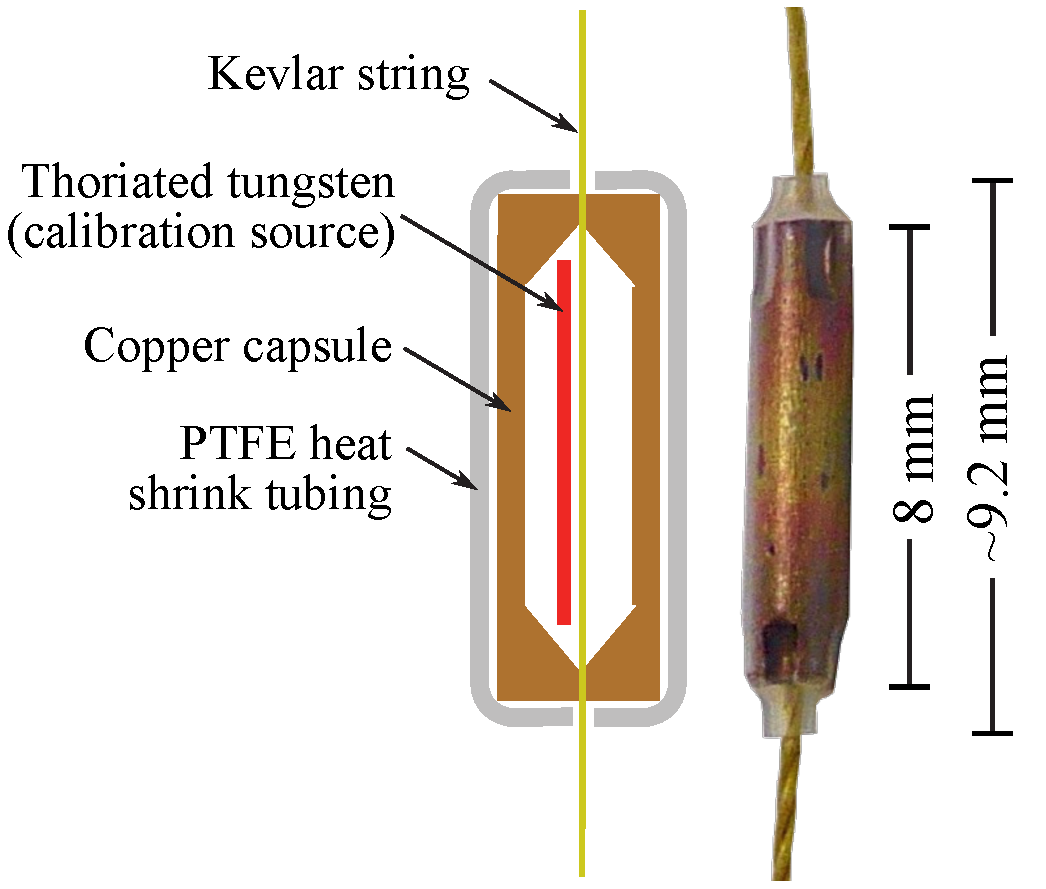
\includegraphics[height=2.2in]{Figures/source_capsule_schematic.pdf}
\caption{}
\label{fig:source_carrierA}
\end{subfigure}
\begin{subfigure}[b]{0.15\textwidth}
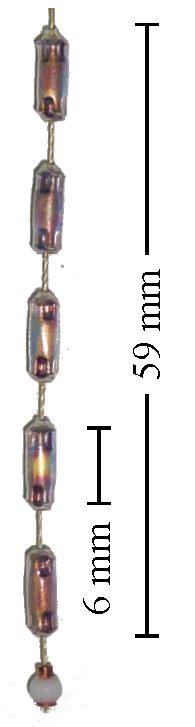
\includegraphics[height=2.7in]{Figures/string_bottom.pdf}
\caption{}
\label{fig:source_carrierB}
\end{subfigure}
\end{center}
\caption[(a) Schematic and photograph of an assembled source capsule. (b) Photograph of five heavier bottom capsules and PTFE ball at the bottom of a source string.]{(a) Schematic and photograph of an assembled source capsule. (b) Photograph of five heavier bottom capsules and PTFE ball at the bottom of a source string.}
\label{fig:source_carrier}
\end{figure}
 

figures to add here: Diagram/picture of source strings, location of source strings in cryostat
\subsection{Motion Boxes}
On top of the cryostat, there are four motion boxes, shown in \autoref{fig:motion_box}, that contain the DCS calibration strings while they are not being deployed. There are three strings in each motion box that are wound up on each of the source string spools in the motion box. These source strings can then be deployed independently and simultaneously down through three guide tubes in the motion box down into the cryostat. A proximity sensor at the bottom of the motion box detects when the copper capsules \color{red} how does the magnet do this? \color{black} are moving either into or out of the motion box. When the DCS is not in operation, the gate valve is closed and the DCS vacuum is disconnected from the rest of the IVC.
\begin{figure}[htpb]
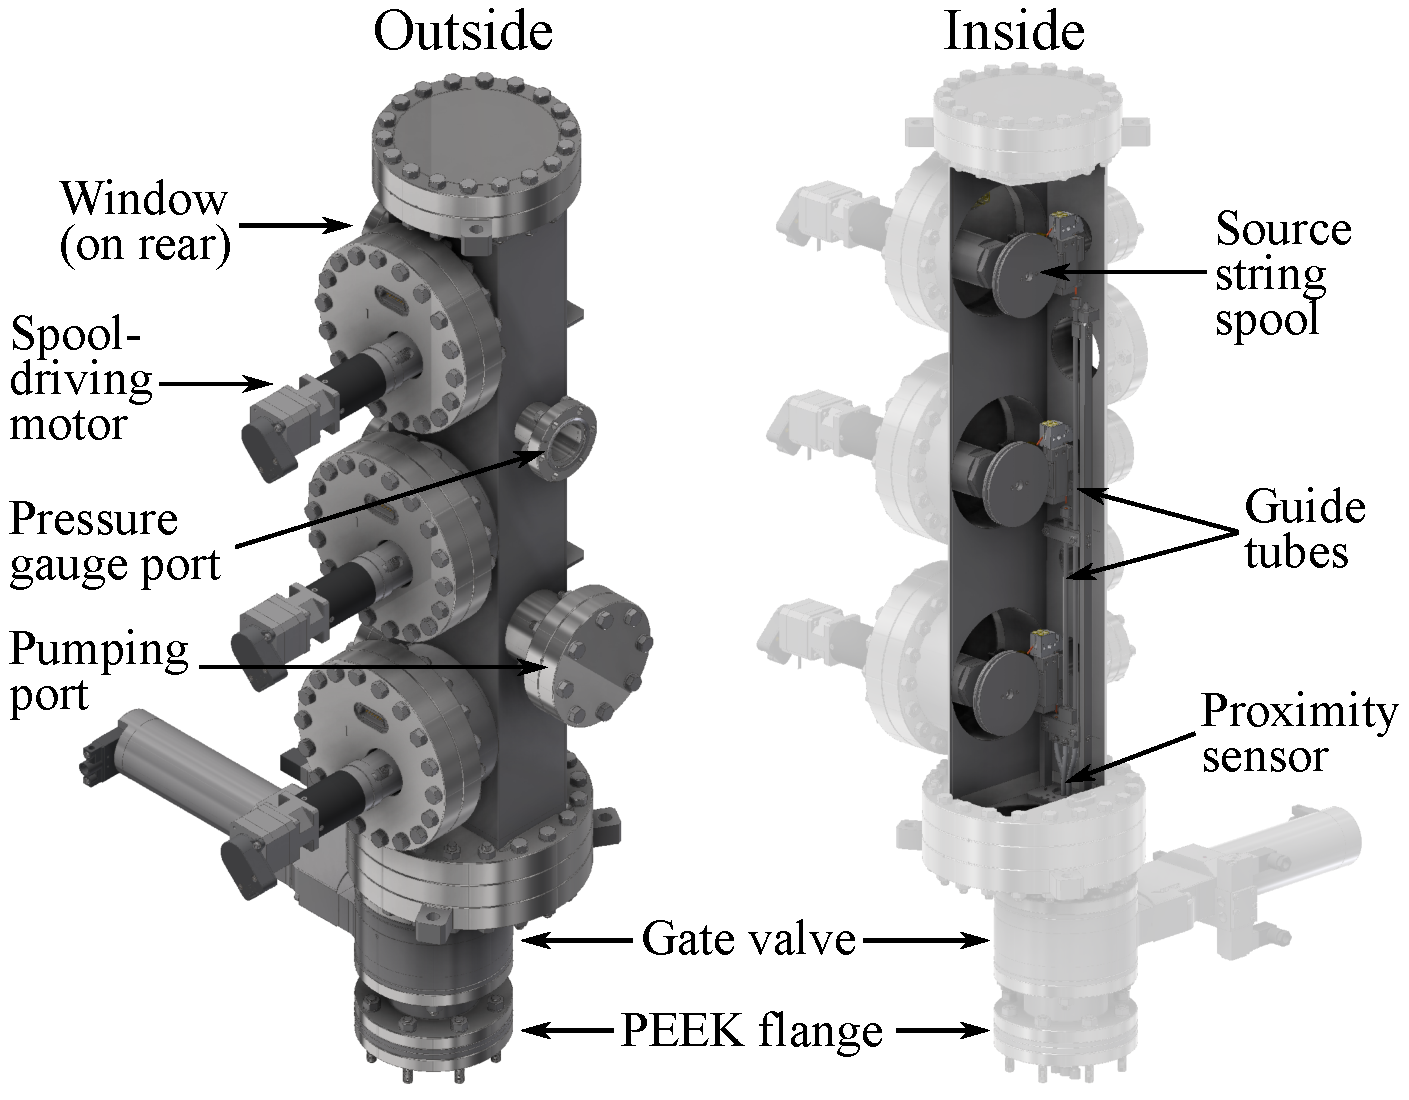
\includegraphics[width=0.9\linewidth]{Figures/motion_box.pdf}
\caption[A rendering of a single motion box from two different angles.]{A rendering of a single motion box from two different angles. The motion box is mounted vertically with the PEEK flange on top of the cryostat with the three source strings spools above. The windows on each motion box allow for the source strings to be observed from outside.}
\label{fig:motion_box}
\end{figure}

\subsection{Thermalization and Thermometry}
In order to deploy 12 calibration source strings from 300 K down to 50 or 10 mK, the sources need to be cooled as much as possible before they reach each stage of the cryostat or even the black-body radiation from the sources will cause the temperature of the crystals and the cryostat to rise excessively and possibly dangerously. Most of the mass, and therefore the heat \color{red} find a better word than heat \color{black} is carried in the copper capsules. The kevlar that holds the capsules is a poor conductor of heat \color{red} Citation Needed \color{black} compared with the capsules, which is a necessary feature, in addition to its strength, as the kevlar will form 12 continuous lines from the motion boxes at 300 K down to the detector region at 10 mK.

To effect this cooling on the source strings, multiple methods are used. The main cooling mechanism used is from the copper thermalizers located at the 4 K plate \color{red} add reference to diagram(s) \color{black}. These thermalizers consist of a moving copper block and a copper base, with the copper block pushed away by a spring. The copper block is activated by another kevlar string that, when pulled, pushes the copper block onto the copper base, applying pressure and a strong \color{red} surely there's a better word to use than strong \color{black} contact with the capsules that are pinned inside. This cooling is performed at the 4K stage as the cryostat has the most cooling power at this stage \color{red} Link to the cooling power table \color{black}. Most of the cooling of the capsules is done at this position and this thermalization process over an entire string is a significant fraction of its total deployment time.

Another way in that heat is removed from the source strings is due to the contact with the walls of the guide tubes. This cooling, however, is limited in two main ways: by the angle of the tube as steeper angles provide less contact with the source capsule and by the heat capacity and thermal contact of the tube with each stage as some tubes, namely those at 600 mK will warm up to 4K or beyond. Below the thermalizers, the inner strings also go through a ``chicane" \color{red} Should I put this in quotes? Also, add reference to figure\color{black} which increases the contact between the capsules and the tubes. This is done to further increase the rate at which heat is removed from the capsules as the cooling on these sources that are to be deployed at the 10 mK stage are the most critical to cool, but the cooling power decreases at colder stages. 

\begin{figure}[htbp]
    \centering
    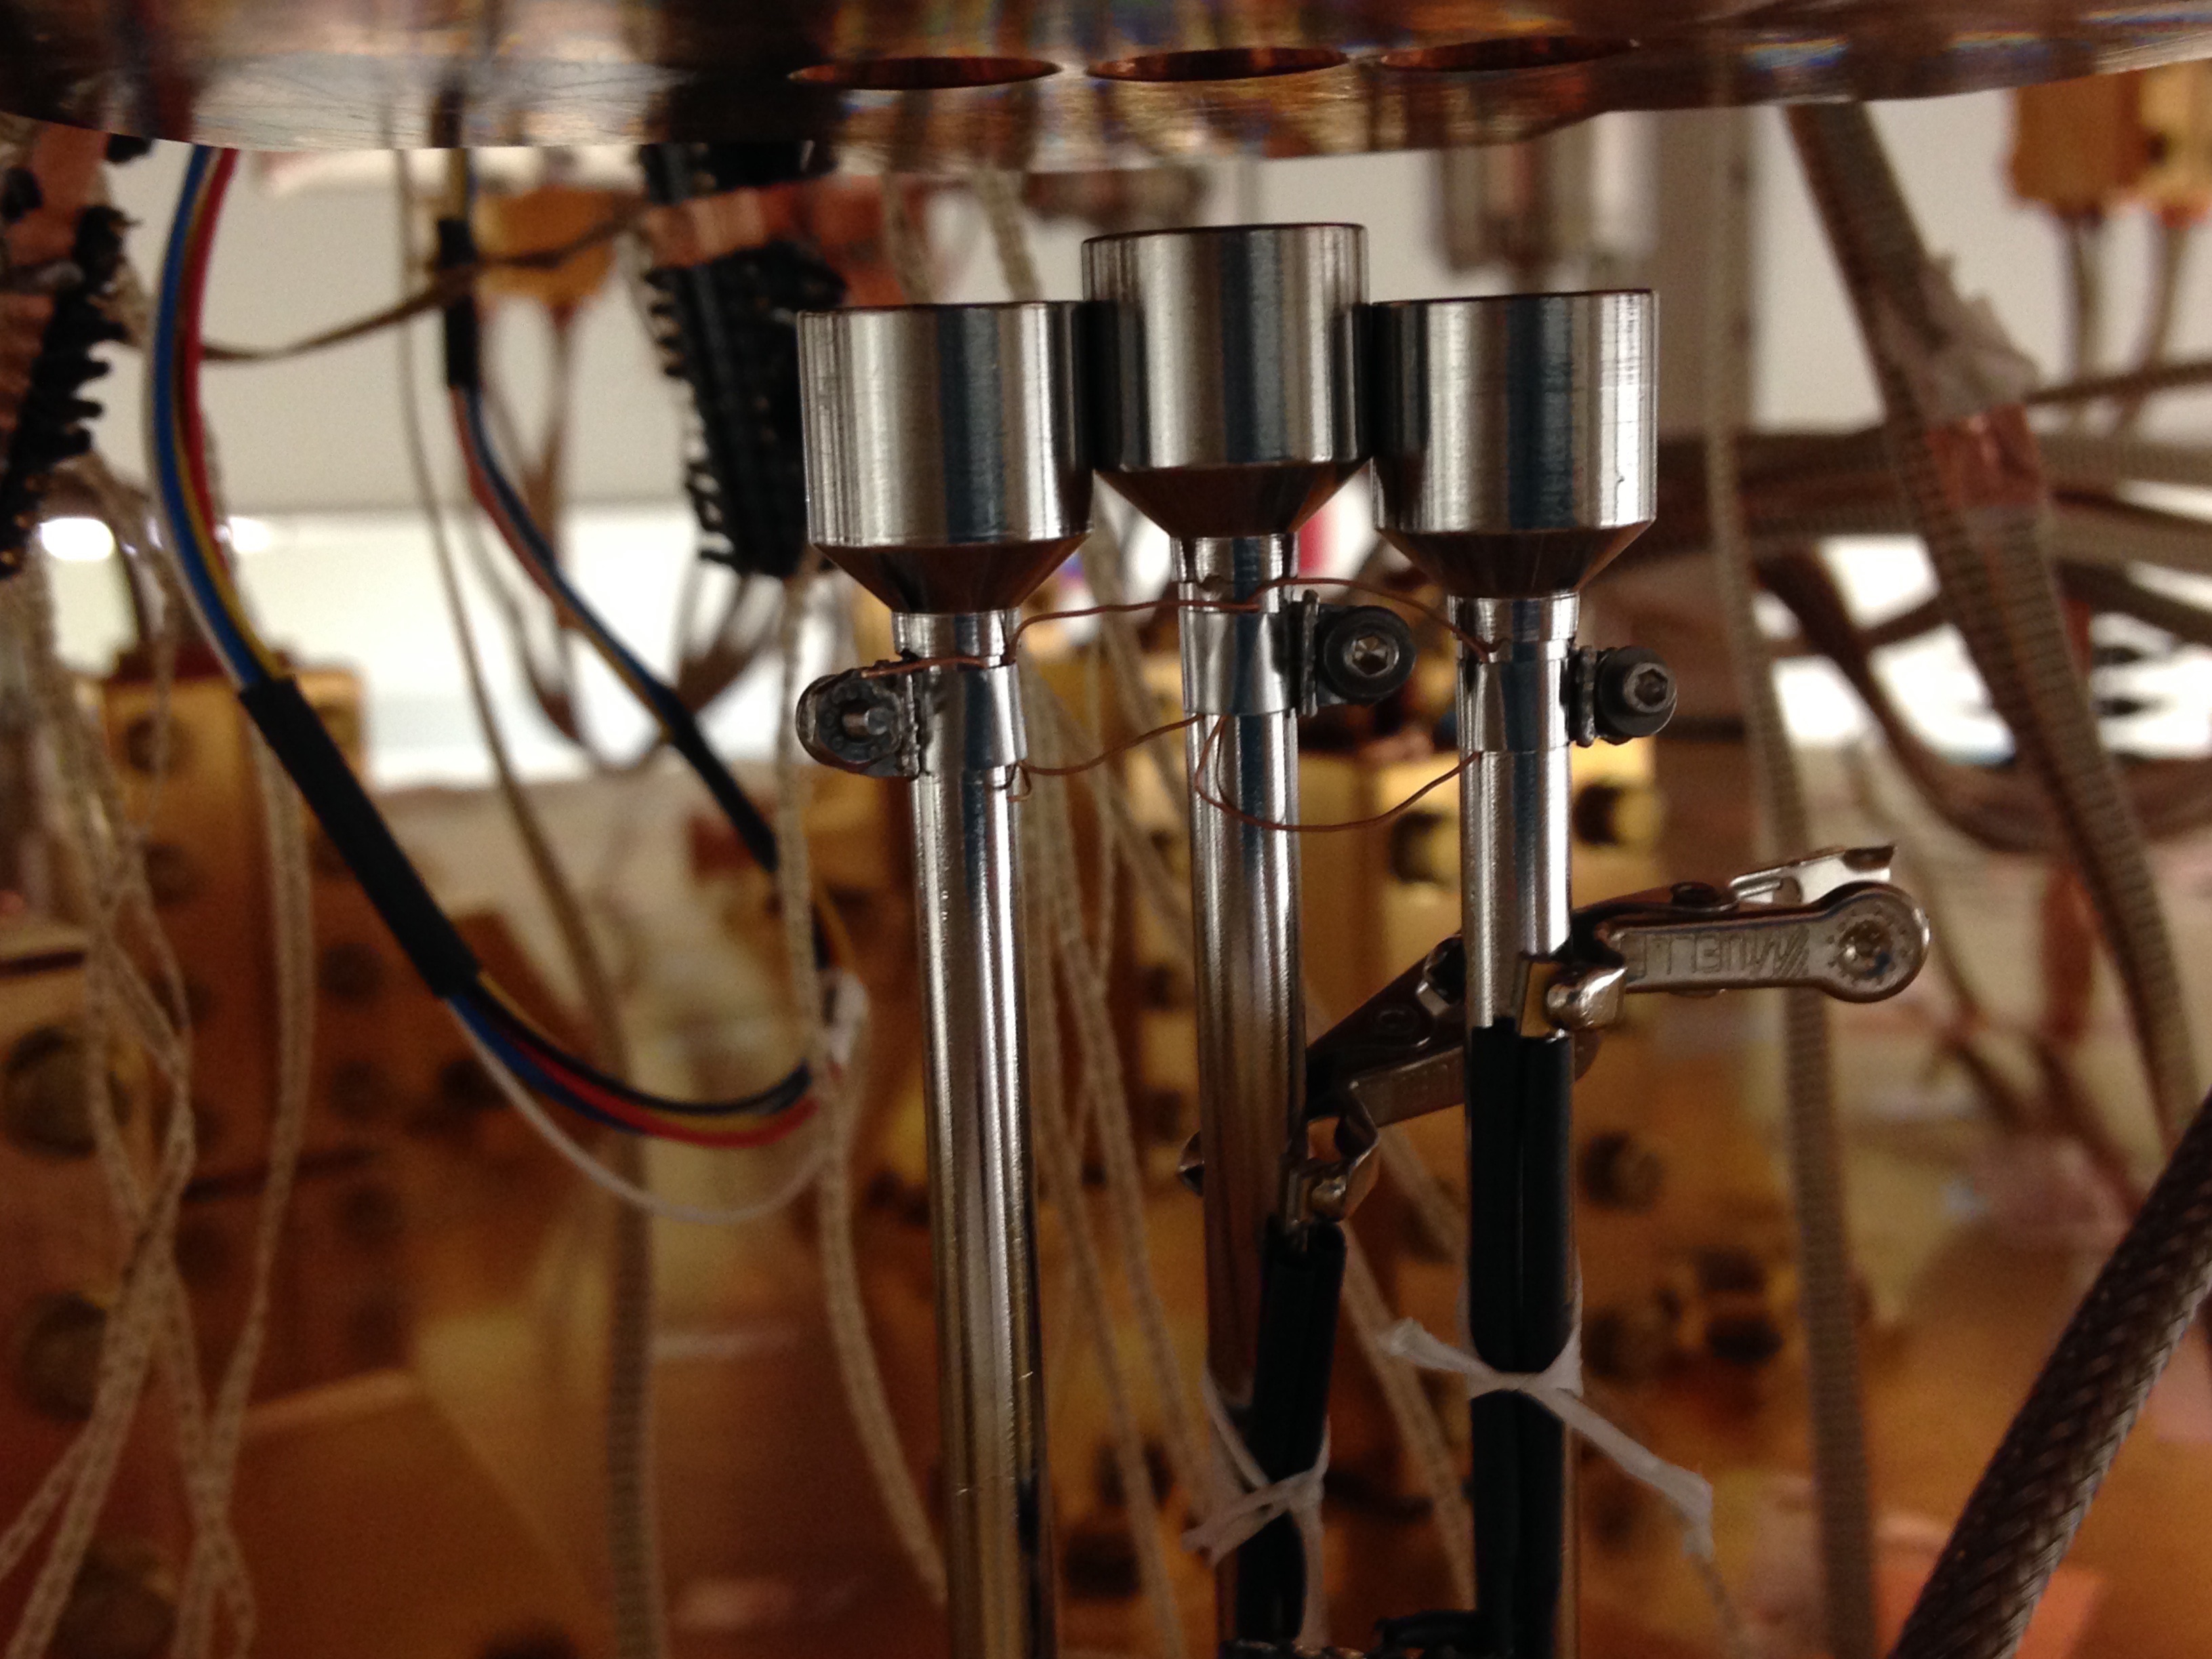
\includegraphics[width=0.8\linewidth]{Figures/ChicaneThermometers.JPG}
    \caption[The chicane thermometers.]
    {The Chicane thermometers under the 4K stage.
    These cernox thermometers are used to determine the temperature of the capsules as they leave the 4~K thermalizer into the 600~mK guide tubes.}
    \label{fig:chicane_thermometers}
\end{figure}

Diagrams to include: pictures of the thermometers, heat loads on the thermometers in different scenarios, 600 mK chicane, 4K thermalizers
\subsection{Impact on Cryostat}

Describe how the calibration affects the state of the cryostat. What are the temperature effects on the plates during the deployment.


\section{Calibration Simulation}
Describe how the simulations for the calibration system are performed. How to determine the best calibration time and effects of pileup.

Figures to include; Geant4 visualization of the sources, rates on the detectors in a calibration, rate dependence on pileup 

\section{Calibration Performance}

Describe how well the calibration system has performed? Also show different strategies for deploying the DCS.

\subsection{Calibration Strategies}

Write about how we go about deploying strings.